% Options for packages loaded elsewhere
\PassOptionsToPackage{unicode}{hyperref}
\PassOptionsToPackage{hyphens}{url}
\PassOptionsToPackage{dvipsnames,svgnames,x11names}{xcolor}
\documentclass[
  10pt,
  a4paper,
]{article}
\usepackage{xcolor}
\usepackage[margin=0.8in]{geometry}
\usepackage{amsmath,amssymb}
\setcounter{secnumdepth}{-\maxdimen} % remove section numbering
\usepackage{iftex}
\ifPDFTeX
  \usepackage[T1]{fontenc}
  \usepackage[utf8]{inputenc}
  \usepackage{textcomp} % provide euro and other symbols
\else % if luatex or xetex
  \usepackage{unicode-math} % this also loads fontspec
  \defaultfontfeatures{Scale=MatchLowercase}
  \defaultfontfeatures[\rmfamily]{Ligatures=TeX,Scale=1}
\fi
\usepackage{lmodern}
\ifPDFTeX\else
  % xetex/luatex font selection
\fi
% Use upquote if available, for straight quotes in verbatim environments
\IfFileExists{upquote.sty}{\usepackage{upquote}}{}
\IfFileExists{microtype.sty}{% use microtype if available
  \usepackage[]{microtype}
  \UseMicrotypeSet[protrusion]{basicmath} % disable protrusion for tt fonts
}{}
\makeatletter
\@ifundefined{KOMAClassName}{% if non-KOMA class
  \IfFileExists{parskip.sty}{%
    \usepackage{parskip}
  }{% else
    \setlength{\parindent}{0pt}
    \setlength{\parskip}{6pt plus 2pt minus 1pt}}
}{% if KOMA class
  \KOMAoptions{parskip=half}}
\makeatother
\usepackage{color}
\usepackage{fancyvrb}
\newcommand{\VerbBar}{|}
\newcommand{\VERB}{\Verb[commandchars=\\\{\}]}
\DefineVerbatimEnvironment{Highlighting}{Verbatim}{commandchars=\\\{\}}
% Add ',fontsize=\small' for more characters per line
\newenvironment{Shaded}{}{}
\newcommand{\AlertTok}[1]{\textcolor[rgb]{1.00,0.00,0.00}{\textbf{#1}}}
\newcommand{\AnnotationTok}[1]{\textcolor[rgb]{0.38,0.63,0.69}{\textbf{\textit{#1}}}}
\newcommand{\AttributeTok}[1]{\textcolor[rgb]{0.49,0.56,0.16}{#1}}
\newcommand{\BaseNTok}[1]{\textcolor[rgb]{0.25,0.63,0.44}{#1}}
\newcommand{\BuiltInTok}[1]{\textcolor[rgb]{0.00,0.50,0.00}{#1}}
\newcommand{\CharTok}[1]{\textcolor[rgb]{0.25,0.44,0.63}{#1}}
\newcommand{\CommentTok}[1]{\textcolor[rgb]{0.38,0.63,0.69}{\textit{#1}}}
\newcommand{\CommentVarTok}[1]{\textcolor[rgb]{0.38,0.63,0.69}{\textbf{\textit{#1}}}}
\newcommand{\ConstantTok}[1]{\textcolor[rgb]{0.53,0.00,0.00}{#1}}
\newcommand{\ControlFlowTok}[1]{\textcolor[rgb]{0.00,0.44,0.13}{\textbf{#1}}}
\newcommand{\DataTypeTok}[1]{\textcolor[rgb]{0.56,0.13,0.00}{#1}}
\newcommand{\DecValTok}[1]{\textcolor[rgb]{0.25,0.63,0.44}{#1}}
\newcommand{\DocumentationTok}[1]{\textcolor[rgb]{0.73,0.13,0.13}{\textit{#1}}}
\newcommand{\ErrorTok}[1]{\textcolor[rgb]{1.00,0.00,0.00}{\textbf{#1}}}
\newcommand{\ExtensionTok}[1]{#1}
\newcommand{\FloatTok}[1]{\textcolor[rgb]{0.25,0.63,0.44}{#1}}
\newcommand{\FunctionTok}[1]{\textcolor[rgb]{0.02,0.16,0.49}{#1}}
\newcommand{\ImportTok}[1]{\textcolor[rgb]{0.00,0.50,0.00}{\textbf{#1}}}
\newcommand{\InformationTok}[1]{\textcolor[rgb]{0.38,0.63,0.69}{\textbf{\textit{#1}}}}
\newcommand{\KeywordTok}[1]{\textcolor[rgb]{0.00,0.44,0.13}{\textbf{#1}}}
\newcommand{\NormalTok}[1]{#1}
\newcommand{\OperatorTok}[1]{\textcolor[rgb]{0.40,0.40,0.40}{#1}}
\newcommand{\OtherTok}[1]{\textcolor[rgb]{0.00,0.44,0.13}{#1}}
\newcommand{\PreprocessorTok}[1]{\textcolor[rgb]{0.74,0.48,0.00}{#1}}
\newcommand{\RegionMarkerTok}[1]{#1}
\newcommand{\SpecialCharTok}[1]{\textcolor[rgb]{0.25,0.44,0.63}{#1}}
\newcommand{\SpecialStringTok}[1]{\textcolor[rgb]{0.73,0.40,0.53}{#1}}
\newcommand{\StringTok}[1]{\textcolor[rgb]{0.25,0.44,0.63}{#1}}
\newcommand{\VariableTok}[1]{\textcolor[rgb]{0.10,0.09,0.49}{#1}}
\newcommand{\VerbatimStringTok}[1]{\textcolor[rgb]{0.25,0.44,0.63}{#1}}
\newcommand{\WarningTok}[1]{\textcolor[rgb]{0.38,0.63,0.69}{\textbf{\textit{#1}}}}
\usepackage{longtable,booktabs,array}
\usepackage{calc} % for calculating minipage widths
% Correct order of tables after \paragraph or \subparagraph
\usepackage{etoolbox}
\makeatletter
\patchcmd\longtable{\par}{\if@noskipsec\mbox{}\fi\par}{}{}
\makeatother
% Allow footnotes in longtable head/foot
\IfFileExists{footnotehyper.sty}{\usepackage{footnotehyper}}{\usepackage{footnote}}
\makesavenoteenv{longtable}
\usepackage{graphicx}
\makeatletter
\newsavebox\pandoc@box
\newcommand*\pandocbounded[1]{% scales image to fit in text height/width
  \sbox\pandoc@box{#1}%
  \Gscale@div\@tempa{\textheight}{\dimexpr\ht\pandoc@box+\dp\pandoc@box\relax}%
  \Gscale@div\@tempb{\linewidth}{\wd\pandoc@box}%
  \ifdim\@tempb\p@<\@tempa\p@\let\@tempa\@tempb\fi% select the smaller of both
  \ifdim\@tempa\p@<\p@\scalebox{\@tempa}{\usebox\pandoc@box}%
  \else\usebox{\pandoc@box}%
  \fi%
}
% Set default figure placement to htbp
\def\fps@figure{htbp}
\makeatother
\setlength{\emergencystretch}{3em} % prevent overfull lines
\providecommand{\tightlist}{%
  \setlength{\itemsep}{0pt}\setlength{\parskip}{0pt}}
\usepackage{bookmark}
\IfFileExists{xurl.sty}{\usepackage{xurl}}{} % add URL line breaks if available
\urlstyle{same}
\hypersetup{
  pdftitle={Indoor Wi-Fi Localization},
  pdfauthor={Kavya Jain; Naman Jain; Dhruv Ramani; Lakshya Agrawal; Akhilesh Kumar},
  colorlinks=true,
  linkcolor={blue},
  filecolor={Maroon},
  citecolor={Blue},
  urlcolor={blue},
  pdfcreator={LaTeX via pandoc}}

\title{Indoor Wi-Fi Localization}
\usepackage{etoolbox}
\makeatletter
\providecommand{\subtitle}[1]{% add subtitle to \maketitle
  \apptocmd{\@title}{\par {\large #1 \par}}{}{}
}
\makeatother
\subtitle{Phase 2: Deep Learning Experiments and Evaluation}
\author{Kavya Jain, Naman Jain, Dhruv Ramani, Lakshya Agrawal, Akhilesh Kumar}
\date{November 2026}

\usepackage{fancyhdr}
\usepackage{float}
\setlength{\headheight}{14pt}
\pagestyle{fancy}
\fancyhf{}
\fancyhead[L]{\small Indoor Wi-Fi Localization}
\fancyhead[R]{\small Phase 2 Report}
\fancyfoot[C]{\thepage}
\renewcommand{\headrulewidth}{0.3pt}
\setlength{\tabcolsep}{3pt}
\renewcommand{\arraystretch}{1.13}
\emergencystretch=2em

\begin{document}
\maketitle

{
\hypersetup{linkcolor=}
\setcounter{tocdepth}{3}
\tableofcontents
}
\section{Abstract}\label{abstract}

This report evaluates neural approaches to building, floor, and
coordinate prediction from Wi-Fi fingerprints in the UJIIndoorLoc
dataset. After removing 637 duplicate training records, 19,300 scans
were assessed using five user-grouped outer folds and three random
seeds. The study compares signal transformations, access-point detection
masks, denoising pretraining, regularization, task sharing, loss
weighting, floor hierarchy, and network capacity. Across the evaluated
multitask designs, independent task networks reached a pooled
out-of-fold EvAAL-style score of 19.29 m and a mean coordinate error of
15.91 m. A controlled width/depth sweep found the lowest mean fold/seed
score with a four-layer, 512-unit architecture (16.68 ± 6.01 m;
coordinate error 13.99 ± 2.95 m). Paired user-level intervals for the
independent versus shared network include zero on the combined score, so
that descriptive ranking is not evidence of a reliable improvement. The
Phase 1 per-building k-nearest-neighbor model remains the stronger
reported coordinate baseline at 12.21 m. Results are from saved Wi-Fi
scans; this report does not claim live localization.

\section{1. Introduction}\label{introduction}

Indoor satellite positioning is unreliable, whereas nearby Wi-Fi access
points provide a repeatable, location-dependent signal pattern.
Fingerprint localization learns the relation between those received
signal strengths (RSSI) and a known reference location. Here a single
scan is mapped to a building identifier, floor identifier, and two
horizontal coordinates. The data and problem setting follow the
UJIIndoorLoc benchmark {[}1{]}. Surveys of Wi-Fi fingerprinting and
neural positioning provide the methodological context {[}2,3{]}. All
numerical findings in this report come from the project's saved
experiments rather than from those surveys.

Phase 1 established classical classifiers and a routed coordinate
estimator. Phase 2 examines whether learned representations and neural
task designs provide useful alternatives under the same user-grouped
evaluation principle. The focus is the trade-off among coordinate
accuracy, building/floor accuracy, and a combined localization penalty.

\section{2. Data and evaluation
design}\label{data-and-evaluation-design}

\subsection{2.1 Dataset and
preprocessing}\label{dataset-and-preprocessing}

UJIIndoorLoc supplies 19,937 training scans and 1,111 official
validation scans. Each record contains 520 ordered wireless access-point
(WAP) readings, building and floor labels, two coordinates, and
collection metadata. The value \texttt{+100} denotes an undetected WAP;
it is not a measured signal. Removing 637 exact duplicate training rows
leaves 19,300 scans. Phase 2 preserves all 520 WAP positions to keep the
neural input layout stable. A detected reading \texttt{r} is clipped to
\texttt{{[}-110,0{]}} dBm before encoding; absence maps to zero.
Coordinate targets are standardized using training users in each fold,
then inverse-transformed to metres for evaluation.

\subsection{2.2 Held-out users and
metrics}\label{held-out-users-and-metrics}

Five deterministic outer GroupKFold partitions are grouped by
\texttt{USERID}; no user appears in both training and assessment
portions of a fold. The three seeds are 42, 1337, and 2024. A complete
model configuration therefore produces 15 fold/seed runs and one
out-of-fold prediction per cleaned scan for each seed. Model selection
and stopping use only outer-training users. The official validation file
is excluded from Phase 2 model selection and from the results below
because it was previously used for a fixed Phase 1 evaluation.

The primary combined measure is the project's EvAAL-style score:

\[S_i=d_i+50\mathbb{1}(\widehat b_i\ne b_i)+4\mathbb{1}(\widehat f_i\ne f_i),\]

where \texttt{d\_i} is Euclidean coordinate error in metres. This score
is a designed penalty, not a physical distance. Building accuracy, floor
accuracy, and unpenalized coordinate error are therefore reported
separately. Pooled out-of-fold values aggregate scans across the three
seeds; mean ± standard deviation across 15 fold/seed runs describes run
variability. These two aggregation methods should not be interchanged.

\section{3. Neural methods}\label{neural-methods}

\subsection{3.1 Signal representation and
missingness}\label{signal-representation-and-missingness}

The linear-positive view maps an observed RSSI \texttt{r} to
\texttt{(clip(r,-110,0)+110)/110}. Additional views use an exponential
map with scale 24 dBm and a power map with exponent \texttt{e}. Each is
evaluated with and without a 520-element binary detection mask. The mask
distinguishes a weak observed signal from an undetected access point.
The six representation configurations share the same 520 → 256 → 128
reference network and were assessed over five folds and three seeds,
giving 90 fold/seed runs.

\subsection{3.2 Denoising pretraining}\label{denoising-pretraining}

A denoising autoencoder has a 520 → 256 → 128 encoder and a mirrored
decoder with sigmoid output for the normalized signal view. On
outer-training users only, observed readings receive Gaussian noise with
4 dBm standard deviation and 10\% access-point dropout. The training
target is the uncorrupted fingerprint. Because roughly 96\% of entries
are absent, reconstruction uses
\texttt{observed\_MSE\ +\ 0.1\ ×\ missing\_MSE} rather than allowing
zero reconstruction to dominate. The trained encoder initializes the
matching supervised reference network; a random initialization provides
the controlled comparison. Each arm has 15 fold/seed runs.

\subsection{3.3 Task architecture and
objective}\label{task-architecture-and-objective}

The principal shared network takes 520 inputs through hidden widths 512,
256, and 128. The first two blocks apply a linear layer, batch
normalization, ReLU, and dropout 0.3; the last uses a linear layer and
ReLU. Its 128-dimensional representation feeds building (128 → 3), floor
(128 → 5), and coordinate (128 → 64 → 2) heads. The default objective is
building cross-entropy + floor cross-entropy + coordinate Huber loss.
Huber loss limits the influence of large coordinate errors relative to
squared loss.

Controlled alternatives use a separate trunk for each task; choose fixed
loss weights from \texttt{(0.5,0.5,2)}, \texttt{(1,1,1)}, and
\texttt{(1,1,2)} within grouped inner validation; learn task uncertainty
weights; or condition floor logits on predicted building probabilities.
The last design uses predicted, never true, building labels during
inference. Training uses AdamW (learning rate \texttt{1e-3}, weight
decay \texttt{1e-4}), batch size 256, at most 200 epochs, patience 20,
and a learning-rate reduction by 0.5 after five non-improving validation
epochs. Grouped inner splits are checked for building-label coverage.
The five distinct task configurations yield 75 fold/seed runs.

\subsection{3.4 Regularization, robustness, and
capacity}\label{regularization-robustness-and-capacity}

A separate 520 → 256 → 128 reference network tests dropout, weight
decay, batch normalization, Gaussian signal noise, and access-point
dropout. The ten configurations produce 150 fold/seed runs. The
reference setting uses dropout 0.2, batch normalization, no weight
decay, Adam at \texttt{1e-3}, batch size 64, and up to 20 epochs with
patience 6. Signal perturbations are applied only to training inputs;
absent WAPs remain absent.

A controlled architecture sweep changes one factor at a time around the
independent-task network with width 512 and depth 3. Depth 2 and 4 are
tested at width 512; width 256 and 1024 are tested at depth 3. The four
new variants contribute 60 fold/seed runs, and the reference reuses 15
existing runs.

\section{4. Experimental results}\label{experimental-results}

\subsection{4.1 Representation and
pretraining}\label{representation-and-pretraining}

\begin{longtable}[]{@{}
  >{\raggedright\arraybackslash}p{(\linewidth - 8\tabcolsep) * \real{0.1579}}
  >{\raggedleft\arraybackslash}p{(\linewidth - 8\tabcolsep) * \real{0.2105}}
  >{\raggedleft\arraybackslash}p{(\linewidth - 8\tabcolsep) * \real{0.2105}}
  >{\raggedleft\arraybackslash}p{(\linewidth - 8\tabcolsep) * \real{0.2105}}
  >{\raggedleft\arraybackslash}p{(\linewidth - 8\tabcolsep) * \real{0.2105}}@{}}
\caption{Comparison of RSSI transformations and detection masks across grouped runs.}\label{tab:phase2_integrated_report-1}\\
\toprule\noalign{}
\begin{minipage}[b]{\linewidth}\raggedright
Signal view
\end{minipage} & \begin{minipage}[b]{\linewidth}\raggedleft
EvAAL-style score (m), mean ± SD
\end{minipage} & \begin{minipage}[b]{\linewidth}\raggedleft
Position error (m)
\end{minipage} & \begin{minipage}[b]{\linewidth}\raggedleft
Building accuracy
\end{minipage} & \begin{minipage}[b]{\linewidth}\raggedleft
Floor accuracy
\end{minipage} \\
\midrule\noalign{}
\endhead
\bottomrule\noalign{}
\endlastfoot
Power + detection mask & \textbf{18.98 ± 2.64} & 17.04 & 97.80\% &
79.18\% \\
Linear + detection mask & 19.47 ± 1.66 & 17.56 & 97.92\% & 78.28\% \\
Exponential + detection mask & 20.35 ± 1.47 & 18.38 & 98.04\% &
75.21\% \\
Linear reference & 21.95 ± 1.71 & 19.40 & 96.31\% & 82.47\% \\
Exponential & 25.65 ± 0.92 & 22.17 & 94.49\% & 81.83\% \\
Power & 29.13 ± 1.38 & 24.66 & 92.50\% & 82.03\% \\
\end{longtable}

The detection mask particularly helps nonlinear signal maps: without it,
a very weak detected reading can become numerically close to an
undetected WAP. The lowest combined score is not uniformly best across
tasks; for example, the masked power view has lower floor accuracy than
the linear reference. In a paired five-fold comparison, the
power-plus-mask view improved the combined score by 2.91 ± 2.28 m
relative to unmasked linear (unadjusted \texttt{p=0.046}). This
exploratory comparison is not adjusted for the six-arm search.

\begin{longtable}[]{@{}
  >{\raggedright\arraybackslash}p{(\linewidth - 6\tabcolsep) * \real{0.2000}}
  >{\raggedleft\arraybackslash}p{(\linewidth - 6\tabcolsep) * \real{0.2667}}
  >{\raggedleft\arraybackslash}p{(\linewidth - 6\tabcolsep) * \real{0.2667}}
  >{\raggedleft\arraybackslash}p{(\linewidth - 6\tabcolsep) * \real{0.2667}}@{}}
\caption{Denoising pretraining versus random initialization.}\label{tab:phase2_integrated_report-2}\\
\toprule\noalign{}
\begin{minipage}[b]{\linewidth}\raggedright
Initialization
\end{minipage} & \begin{minipage}[b]{\linewidth}\raggedleft
EvAAL-style score (m), mean ± SD
\end{minipage} & \begin{minipage}[b]{\linewidth}\raggedleft
Position error (m)
\end{minipage} & \begin{minipage}[b]{\linewidth}\raggedleft
Floor accuracy
\end{minipage} \\
\midrule\noalign{}
\endhead
\bottomrule\noalign{}
\endlastfoot
Random & 21.95 ± 1.71 & 19.40 & 82.50\% \\
Denoising-pretrained encoder & \textbf{19.76 ± 0.87} & \textbf{17.42} &
82.13\% \\
\end{longtable}

Pretraining lowers the pooled localization errors in the current runs.
In a paired user-cluster analysis, its mean user-level combined-score
difference versus random initialization is −1.32 m (95\% percentile
interval −2.48 to −0.39 m); floor accuracy is lower by 1.1 percentage
points (−2.0 to −0.3 points). The comparisons are exploratory and
unadjusted for multiple model tests.

\subsection{4.2 Task design}\label{task-design}

\begin{longtable}[]{@{}
  >{\raggedright\arraybackslash}p{(\linewidth - 8\tabcolsep) * \real{0.1579}}
  >{\raggedleft\arraybackslash}p{(\linewidth - 8\tabcolsep) * \real{0.2105}}
  >{\raggedleft\arraybackslash}p{(\linewidth - 8\tabcolsep) * \real{0.2105}}
  >{\raggedleft\arraybackslash}p{(\linewidth - 8\tabcolsep) * \real{0.2105}}
  >{\raggedleft\arraybackslash}p{(\linewidth - 8\tabcolsep) * \real{0.2105}}@{}}
\caption{Pooled out-of-fold comparison of neural task designs.}\label{tab:phase2_integrated_report-3}\\
\toprule\noalign{}
\begin{minipage}[b]{\linewidth}\raggedright
Network design
\end{minipage} & \begin{minipage}[b]{\linewidth}\raggedleft
Pooled EvAAL-style score (m)
\end{minipage} & \begin{minipage}[b]{\linewidth}\raggedleft
Pooled position error (m)
\end{minipage} & \begin{minipage}[b]{\linewidth}\raggedleft
Building accuracy
\end{minipage} & \begin{minipage}[b]{\linewidth}\raggedleft
Floor accuracy
\end{minipage} \\
\midrule\noalign{}
\endhead
\bottomrule\noalign{}
\endlastfoot
Independent task networks & \textbf{19.29} & \textbf{15.91} & 94.66\% &
\textbf{82.18\%} \\
Selected fixed loss weights & 20.11 & 17.66 & \textbf{96.61\%} &
81.23\% \\
Shared equal-weight network & 21.47 & 18.67 & 95.85\% & 81.86\% \\
Building-conditioned floor head & 22.00 & 19.36 & 96.20\% & 81.42\% \\
Learned uncertainty weights & 22.25 & 19.66 & 96.34\% & 81.03\% \\
\end{longtable}

Independent trunks produce the lowest observed combined score and
coordinate error among the task-design variants, whereas selected fixed
weights yield higher building accuracy. This is consistent with task
interference in a shared representation but does not by itself prove
that sharing is harmful across datasets. Relative to the shared network,
the independent network's paired user-level combined-score difference is
−1.11 m (95\% interval −2.76 to 0.38 m). The interval includes zero. Its
position-error difference is −1.66 m (−3.11 to −0.47 m). These intervals
use 2,000 resamples of 18 user clusters; they are exploratory and
unadjusted for multiple comparisons.

\begin{figure}[H]
\centering
\pandocbounded{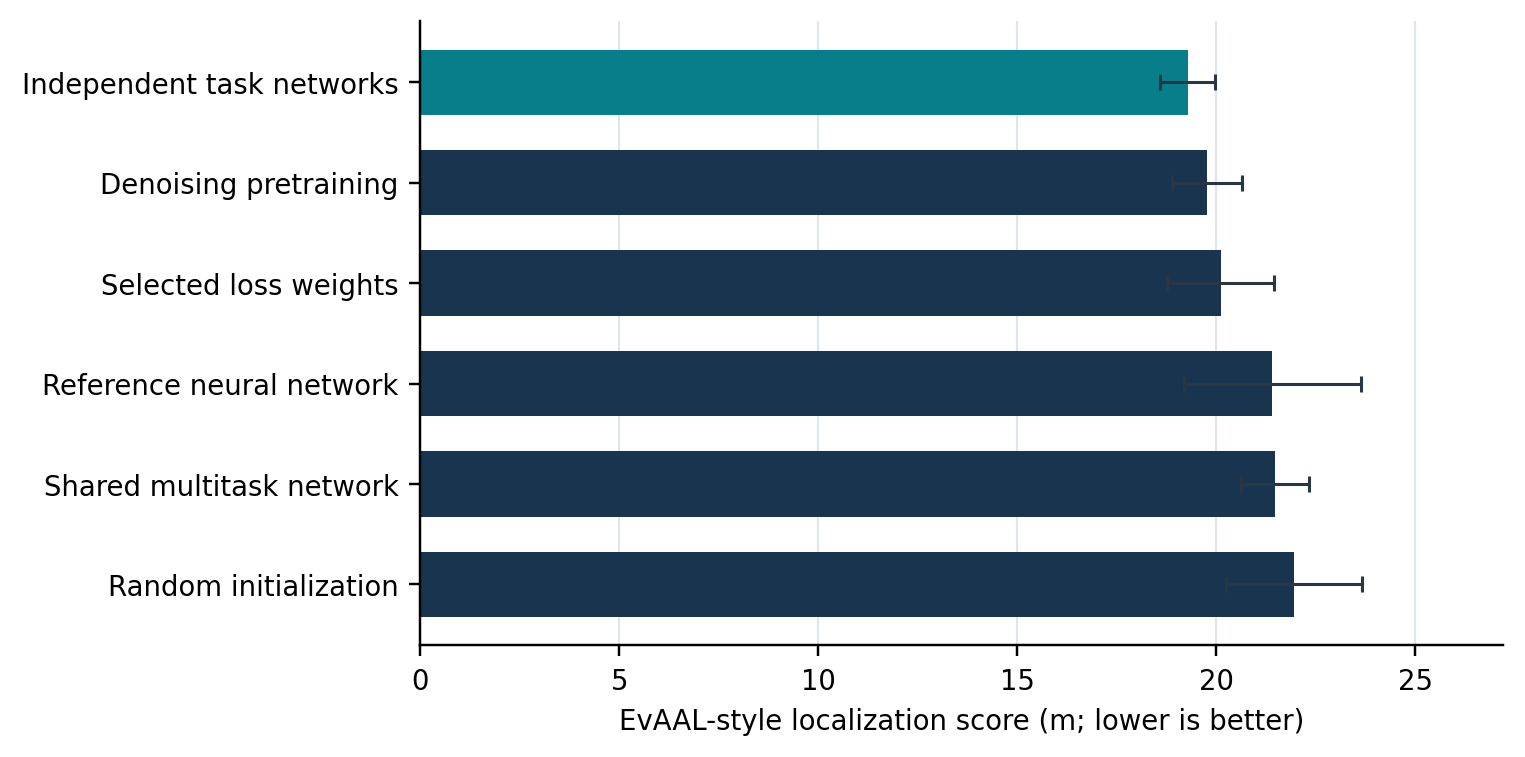
\includegraphics[keepaspectratio,alt={Comparison of evaluated neural pipelines on pooled out-of-fold scans. Error bars show between-seed variation.}]{../results/figures/report_model_comparison.png}}
\caption{Comparison of evaluated neural pipelines on pooled out-of-fold
scans. Error bars show between-seed variation.}
\end{figure}

\subsection{4.3 Network width and depth}\label{network-width-and-depth}

\begin{longtable}[]{@{}
  >{\raggedright\arraybackslash}p{(\linewidth - 8\tabcolsep) * \real{0.1579}}
  >{\raggedleft\arraybackslash}p{(\linewidth - 8\tabcolsep) * \real{0.2105}}
  >{\raggedleft\arraybackslash}p{(\linewidth - 8\tabcolsep) * \real{0.2105}}
  >{\raggedleft\arraybackslash}p{(\linewidth - 8\tabcolsep) * \real{0.2105}}
  >{\raggedleft\arraybackslash}p{(\linewidth - 8\tabcolsep) * \real{0.2105}}@{}}
\caption{Controlled network width and depth comparison across fold and seed runs.}\label{tab:phase2_integrated_report-4}\\
\toprule\noalign{}
\begin{minipage}[b]{\linewidth}\raggedright
Hidden width × depth
\end{minipage} & \begin{minipage}[b]{\linewidth}\raggedleft
Combined score (m), mean ± SD
\end{minipage} & \begin{minipage}[b]{\linewidth}\raggedleft
Position error (m), mean ± SD
\end{minipage} & \begin{minipage}[b]{\linewidth}\raggedleft
Building accuracy
\end{minipage} & \begin{minipage}[b]{\linewidth}\raggedleft
Floor accuracy
\end{minipage} \\
\midrule\noalign{}
\endhead
\bottomrule\noalign{}
\endlastfoot
512 × 2 & 20.95 ± 7.18 & 17.30 ± 4.16 & 94.29\% ± 8.11\% & 80.02\% ±
12.87\% \\
512 × 3 reference & 19.29 ± 6.31 & 15.84 ± 2.63 & 94.56\% ± 8.02\% &
81.82\% ± 12.60\% \\
512 × 4 & \textbf{16.68 ± 6.01} & \textbf{13.99 ± 2.95} &
\textbf{96.06\% ± 6.24\%} & \textbf{82.01\% ± 11.18\%} \\
256 × 3 & 21.31 ± 6.83 & 18.47 ± 4.51 & 95.84\% ± 6.63\% & 80.96\% ±
12.34\% \\
1024 × 3 & 17.71 ± 6.79 & 14.23 ± 3.26 & 94.53\% ± 8.48\% & 81.49\% ±
10.23\% \\
\end{longtable}

The four-layer, 512-unit model has the lowest mean score across the 15
fold/seed runs in this controlled sweep. The table reports run-level
mean ± sample standard deviation, whereas the preceding task-design
table reports pooled scan-level values. The capacity result is a
descriptive ranking; no user-cluster paired interval is reported for
this width/depth comparison.

\begin{figure}[H]
\centering
\pandocbounded{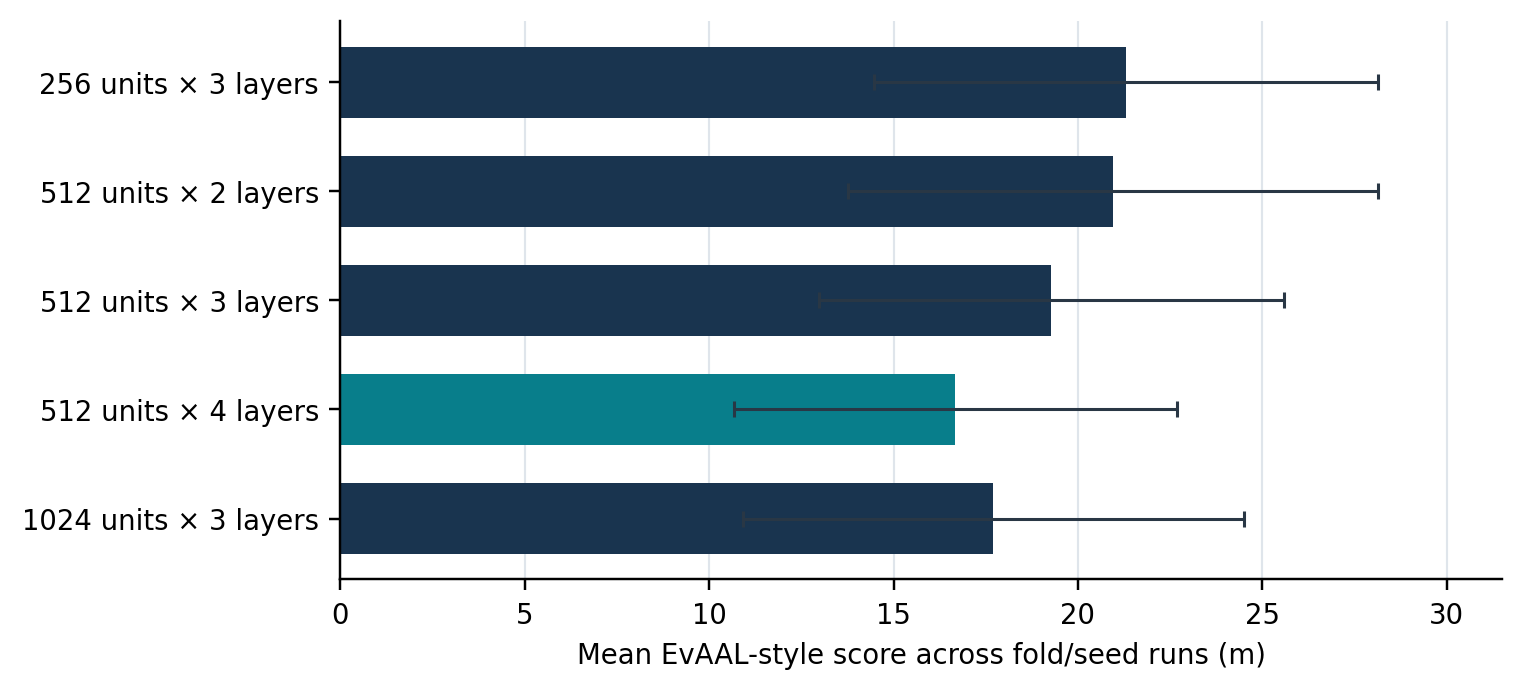
\includegraphics[keepaspectratio,alt={Mean combined localization score for the controlled width and depth sweep. Error bars represent variation across fold/seed runs.}]{../results/figures/report_architecture_capacity.png}}
\caption{Mean combined localization score for the controlled width and
depth sweep. Error bars represent variation across fold/seed runs.}
\end{figure}

\subsection{4.4 Data-volume and calibration
diagnostics}\label{data-volume-and-calibration-diagnostics}

The independent-task architecture was retrained on 25\%, 50\%, 75\%, and
100\% of each outer-training partition while retaining the same held-out
users. The epoch count selected for the corresponding full-data run was
held fixed across fractions, so this is a training-volume comparison
under a fixed schedule.

\begin{longtable}[]{@{}
  >{\raggedleft\arraybackslash}p{(\linewidth - 6\tabcolsep) * \real{0.2500}}
  >{\raggedleft\arraybackslash}p{(\linewidth - 6\tabcolsep) * \real{0.2500}}
  >{\raggedleft\arraybackslash}p{(\linewidth - 6\tabcolsep) * \real{0.2500}}
  >{\raggedleft\arraybackslash}p{(\linewidth - 6\tabcolsep) * \real{0.2500}}@{}}
\caption{Learning curve under a fixed training schedule.}\label{tab:phase2_integrated_report-5}\\
\toprule\noalign{}
\begin{minipage}[b]{\linewidth}\raggedleft
Training fraction
\end{minipage} & \begin{minipage}[b]{\linewidth}\raggedleft
Mean training scans
\end{minipage} & \begin{minipage}[b]{\linewidth}\raggedleft
Combined score (m), mean ± SD
\end{minipage} & \begin{minipage}[b]{\linewidth}\raggedleft
Position error (m), mean ± SD
\end{minipage} \\
\midrule\noalign{}
\endhead
\bottomrule\noalign{}
\endlastfoot
25\% & 3,860 & 26.41 ± 11.71 & 24.24 ± 12.14 \\
50\% & 7,720 & 21.01 ± 6.54 & 17.98 ± 5.13 \\
75\% & 11,580 & 18.96 ± 6.49 & 16.24 ± 4.47 \\
100\% & 15,440 & 19.29 ± 6.31 & 15.84 ± 2.63 \\
\end{longtable}

Position error falls as more data are used in this sweep, although the
combined score is not perfectly monotonic between 75\% and 100\%.
Variation across folds and seeds remains substantial.

\begin{figure}[H]
\centering
\pandocbounded{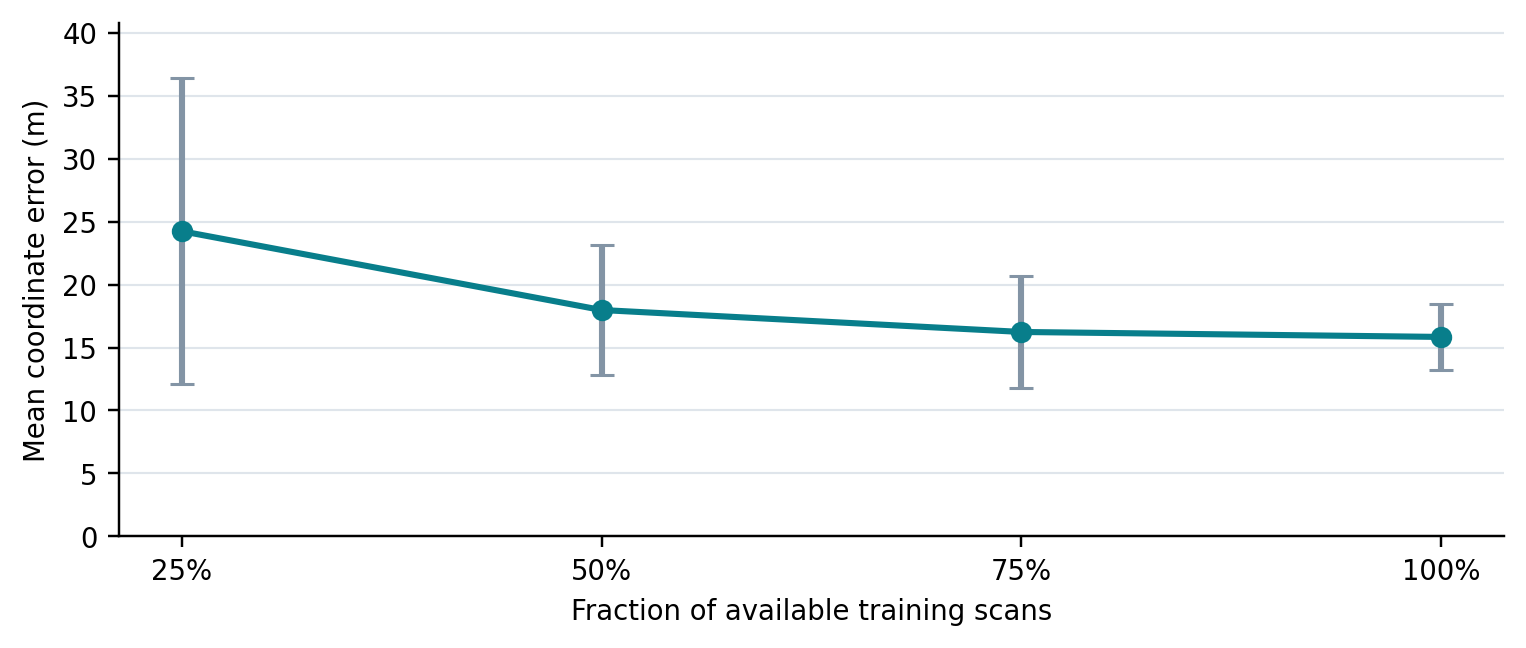
\includegraphics[keepaspectratio,alt={Coordinate error as the amount of training data increases. Error bars show fold/seed variation.}]{../results/figures/report_learning_curve.png}}
\caption{Coordinate error as the amount of training data increases.
Error bars show fold/seed variation.}
\end{figure}

Floor probabilities were assessed on held-out folds using 15-bin
expected calibration error (ECE), multiclass Brier score, and negative
log-likelihood. The independent and shared networks both have floor ECE
near 0.139, but the independent network's negative log-likelihood is
1.503 versus 1.261 for the shared network. Thus better floor-label
accuracy does not necessarily imply better probability quality. ECE is
sensitive to bin choice and is read alongside the proper scoring rules.

\section{5. Interpretation and study
limitations}\label{interpretation-and-study-limitations}

The strongest reported Phase 1 coordinate result is 12.21 m mean error
for tuned per-building k-nearest neighbors using predicted building
routing. The best architecture in the Phase 2 width/depth sweep has a
13.99 m mean run-level position error. These estimates come from related
user-grouped experiments but from different model families and
aggregation summaries. The measured Phase 2 neural results therefore do
not establish a coordinate-accuracy improvement over the classical
baseline. The neural study instead supplies controlled evidence about
representation, task design, and capacity.

The robustness sweep uses a smaller reference network than the principal
task-design and capacity experiments. Its comparisons are valid within
that sweep, but the changes cannot be isolated from architecture when
compared with the larger models. Two outer folds in that sweep have
limited building-label coverage in the inner stopping split; this
affects the reliability of the selected stopping epoch, although their
outer assessment users remain held out. The benchmark has only 18 user
groups after cleaning, so uncertainty is better estimated by
user-cluster resampling than by treating individual scans as
independent. The bootstrap intervals are unadjusted across many
comparisons. The official validation file was previously used for a
Phase 1 baseline and is not treated as fresh independent confirmation.
Finally, the data consist of recorded fingerprints from the benchmark
buildings; the project does not establish performance on a new building,
phone fleet, or live scan.

\section{6. Reproducibility}\label{reproducibility}

The repository pins Python dependencies and stores fold definitions,
per-run records, out-of-fold predictions, aggregate CSV tables, and
generated figures. The raw UJIIndoorLoc CSV files are downloaded
separately. From the repository root, the environment and saved-data
audit can be prepared with:

\begin{Shaded}
\begin{Highlighting}[]
\ExtensionTok{python3.11} \AttributeTok{{-}m}\NormalTok{ venv .venv}
\BuiltInTok{source}\NormalTok{ .venv/bin/activate}
\ExtensionTok{python} \AttributeTok{{-}m}\NormalTok{ pip install }\AttributeTok{{-}r}\NormalTok{ requirements.txt}
\ExtensionTok{python}\NormalTok{ scripts/download\_data.py}
\ExtensionTok{python}\NormalTok{ scripts/build\_splits.py}
\ExtensionTok{pytest}
\ExtensionTok{python}\NormalTok{ scripts/build\_publication\_figures.py}
\end{Highlighting}
\end{Shaded}

The report figures are generated from saved CSV summaries in
\texttt{results/phase2/}; the images are under
\texttt{results/figures/}. Training runners and their parameters are
recorded in the repository source and per-run JSON files. Regenerating
all 15-run experiment grids requires substantially more computation than
rebuilding this report from the saved artifacts.

\section{7. Conclusion}\label{conclusion}

The evaluated neural systems can jointly predict a building, floor, and
coordinates from a fixed 520-WAP fingerprint. An explicit detection mask
improves several nonlinear RSSI views, denoising pretraining improves
the measured reference localization score with a floor-accuracy
trade-off, and independent task networks give the lowest observed pooled
score among the principal task-design variants. A deeper 512-unit
network gives the lowest descriptive score in the capacity sweep. Paired
uncertainty and the stronger Phase 1 coordinate baseline constrain the
interpretation: the study identifies useful model-design effects without
demonstrating that Phase 2 surpasses the classical model in coordinate
accuracy.

\section{References}\label{references}

\begin{enumerate}
\def\labelenumi{\arabic{enumi}.}
\tightlist
\item
  UCI Machine Learning Repository, ``UJIIndoorLoc,'' DOI:
  \href{https://doi.org/10.24432/C5MS59}{10.24432/C5MS59}.
\item
  S. Xia, Y. Liu, G. Yuan, M. Zhu, and Z. Wang, ``Indoor Fingerprint
  Positioning Based on Wi-Fi: An Overview,'' \emph{ISPRS International
  Journal of Geo-Information}, 6(5), 135, 2017, DOI:
  \href{https://doi.org/10.3390/ijgi6050135}{10.3390/ijgi6050135}.
\item
  X. Feng, K. A. Nguyen, and Z. Luo, ``A survey of deep learning
  approaches for WiFi-based indoor positioning,'' \emph{Journal of
  Information and Telecommunication}, 6(2), 163--216, 2022, DOI:
  \url{https://doi.org/10.1080/24751839.2021.1975425}.
\end{enumerate}

\end{document}
